\section{Конструкторский раздел}
%В этом разделе будет приведено проектирование базы данных и проектирование приложения.
%Также будет спроектирован триггер, осуществляющие автоматически пересчитывать рейтинга турнира при добавлении новых оценок.

\subsection{Алгоритм составления расписания турнира}

Условием организации футбольного турнира является то, что количество участвующих команд должно быть четным.

Турнирное расписание матчей для набора команд , удовлетворяющее приведенному ниже набору ограничений:
\begin{itemize}
	\item ни одна команда не должна играть 2 матча подряд в одной неделе;
	\item каждая команда должна была играть ровно 2 матча со всеми остальными командами. Второй матч состоится после встречи всех оставшихся команд;
	\item интервал между двумя матчами равен неделе.
\end{itemize}

На рисунке \ref{img:schedule} приведена схема алгоритма составления расписания турнира.

\begin{figure}[h]
	\centering
	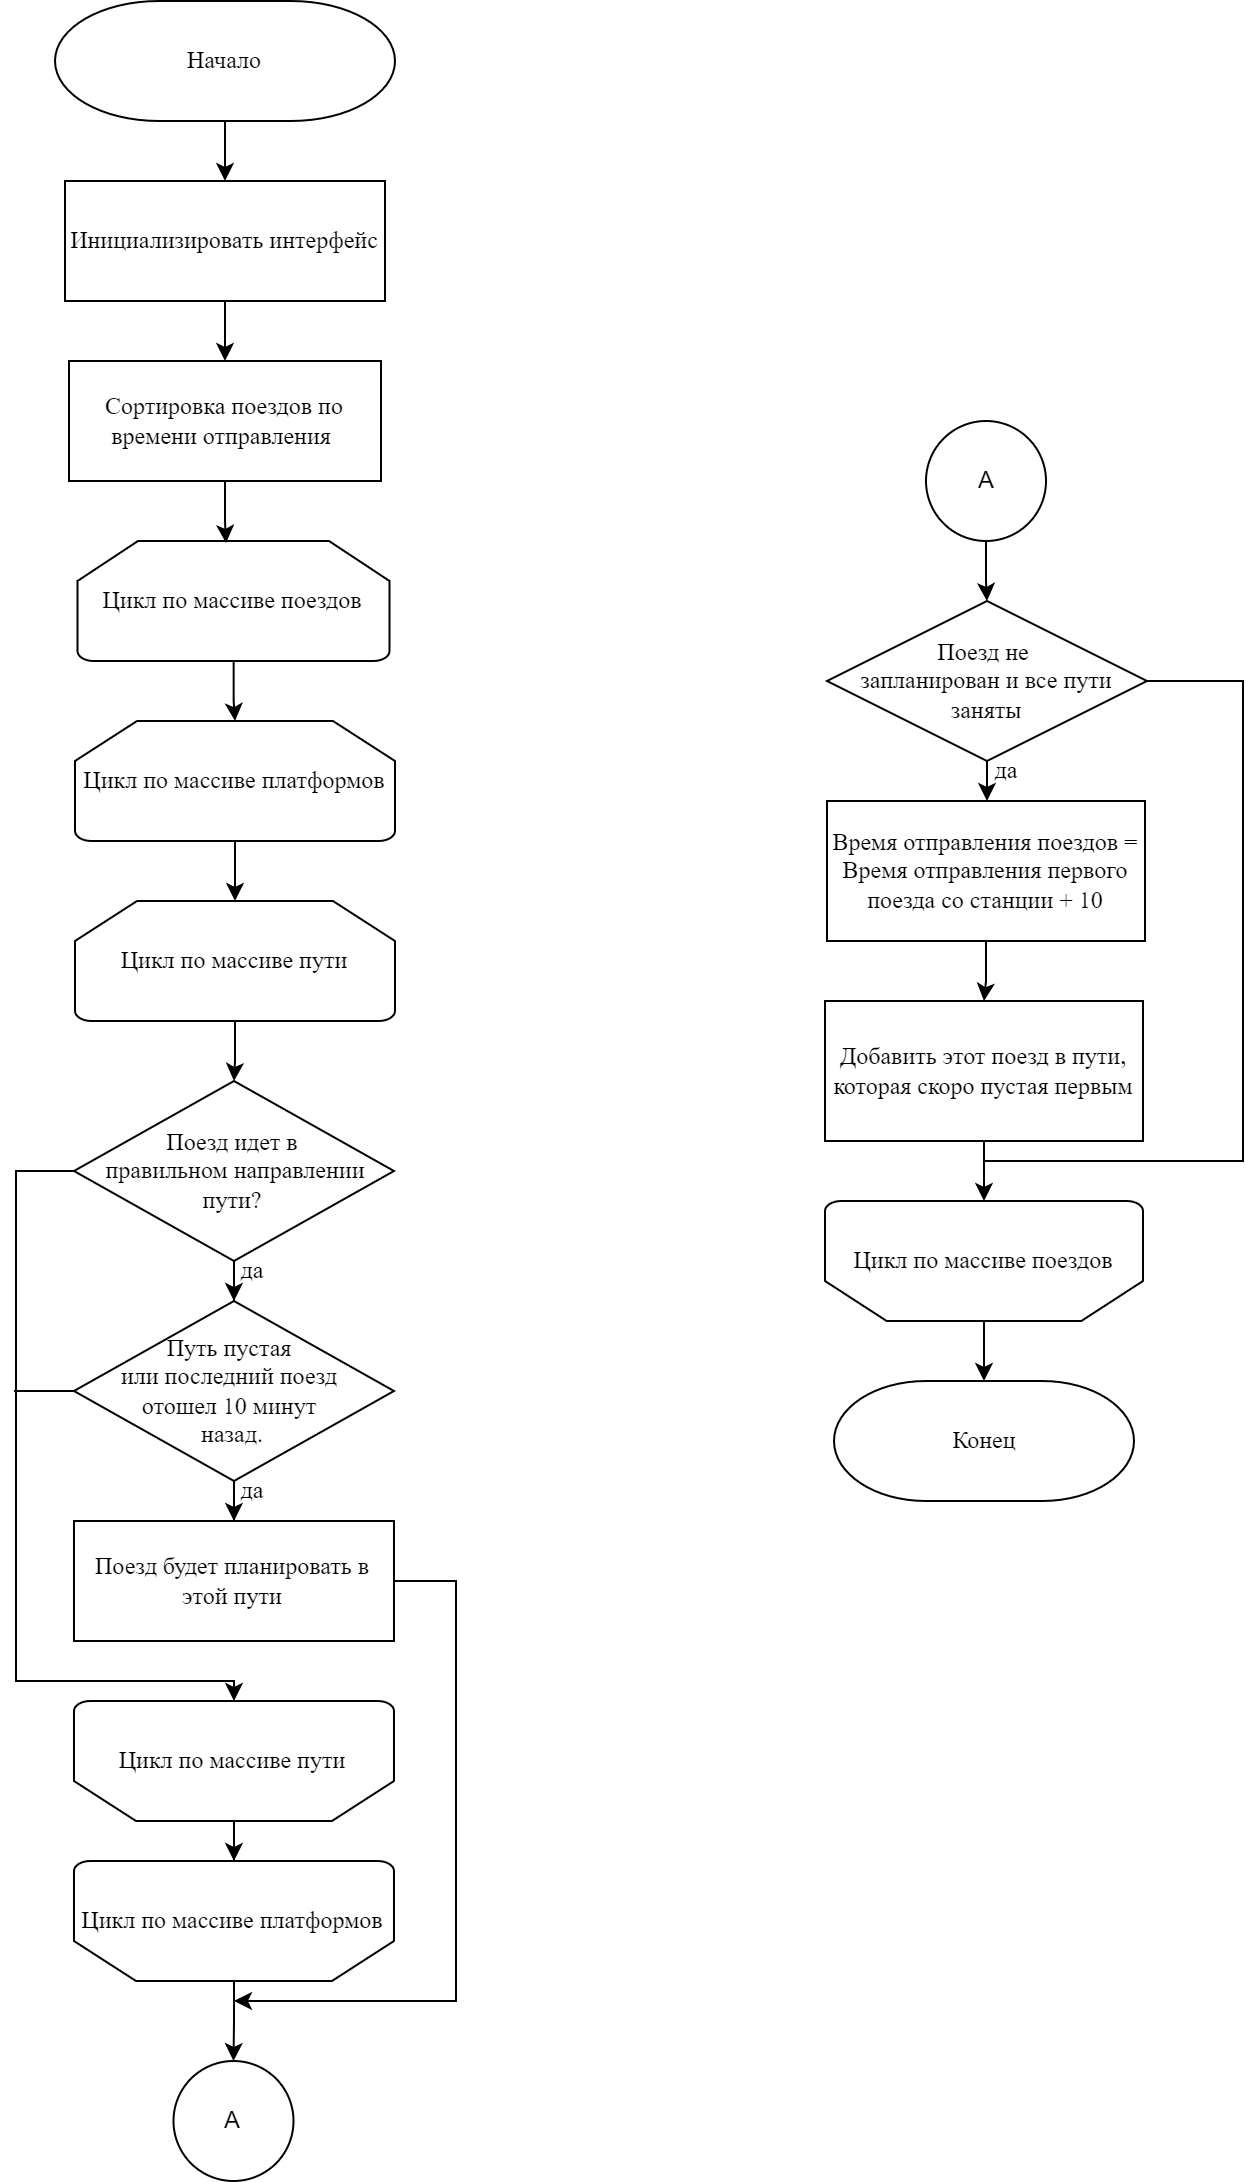
\includegraphics[height=0.45\textheight]{img/schedule.png}
	\caption{Алгоритм составления расписания турнира}
	\label{img:schedule}
\end{figure}
\clearpage

\subsection*{Вывод}
Были приведено проектирование базы данных и проектирование приложения.
Был спроектирован триггер, осуществляющие автоматически пересчитывать рейтинга турнира при добавлении новых оценок.
Также была приведена схема алгоритма составления расписания турнира.